%%%%%%%%%%%%%%%%%%%%%%%%%%%%%%%%%%%%%%%%%%%%%%%%%%%%%%%%%%%%%%%%%%%%%%%%%%%%%%%%
% Template for USENIX papers.
%
% History:
%
% - TEMPLATE for Usenix papers, specifically to meet requirements of
%   USENIX '05. originally a template for producing IEEE-format
%   articles using LaTeX. written by Matthew Ward, CS Department,
%   Worcester Polytechnic Institute. adapted by David Beazley for his
%   excellent SWIG paper in Proceedings, Tcl 96. turned into a
%   smartass generic template by De Clarke, with thanks to both the
%   above pioneers. Use at your own risk. Complaints to /dev/null.
%   Make it two column with no page numbering, default is 10 point.
%
% - Munged by Fred Douglis <douglis@research.att.com> 10/97 to
%   separate the .sty file from the LaTeX source template, so that
%   people can more easily include the .sty file into an existing
%   document. Also changed to more closely follow the style guidelines
%   as represented by the Word sample file.
%
% - Note that since 2010, USENIX does not require endnotes. If you
%   want foot of page notes, don't include the endnotes package in the
%   usepackage command, below.
% - This version uses the latex2e styles, not the very ancient 2.09
%   stuff.
%
% - Updated July 2018: Text block size changed from 6.5" to 7"
%
% - Updated Dec 2018 for ATC'19:
%
%   * Revised text to pass HotCRP's auto-formatting check, with
%     hotcrp.settings.submission_form.body_font_size=10pt, and
%     hotcrp.settings.submission_form.line_height=12pt
%
%   * Switched from \endnote-s to \footnote-s to match Usenix's policy.
%
%   * \section* => \begin{abstract} ... \end{abstract}
%
%   * Make template self-contained in terms of bibtex entires, to allow
%     this file to be compiled. (And changing refs style to 'plain'.)
%
%   * Make template self-contained in terms of figures, to
%     allow this file to be compiled. 
%
%   * Added packages for hyperref, embedding fonts, and improving
%     appearance.
%   
%   * Removed outdated text.
%
%%%%%%%%%%%%%%%%%%%%%%%%%%%%%%%%%%%%%%%%%%%%%%%%%%%%%%%%%%%%%%%%%%%%%%%%%%%%%%%%

\documentclass[letterpaper,twocolumn,10pt]{article}
\usepackage{usenix2019_v3}

% to be able to draw some self-contained figs
\usepackage{tikz}
\usepackage{amsmath}

% inlined bib file
\usepackage{filecontents}



%-------------------------------------------------------------------------------
\begin{document}
%-------------------------------------------------------------------------------

%don't want date printed
\date{}

% make title bold and 14 pt font (Latex default is non-bold, 16 pt)
\title{\Large \bf Ghidra Decompiler}

%for single author (just remove % characters)
\author{
{\rm Daniel Ebert 65926}\\
Hochschule Aalen - Penetration Testing und Computerforensik
}

\maketitle
% TODO: bücher references von tobias arnold?
% TODO: grammarcheck via word!

\begin{abstract}

In diesem Handout wird die Funktionsweise des Ghidra Decompilers und dessen Einsatz erläutert. Der Ghidra Decompiler übersetzt Maschinencode zu lesbarem C-ähnlichen Code \cite{8}. Ein Reverse Engineer kann den Ghidra Decompiler einsetzen, wenn der originale Source Code für ein Binary nicht zur Verfügung steht. Der Higher-Level C-ähnliche Code hilft dem Reverse Engineer dabei, die Funktionsweise des Codes schneller zu verstehen. Der Decompiler automatisiert nicht die Fehlererkennung. Allerdings vereinfacht der Decompiler den Prozess Fehler zu erkennen für den Benutzer. Ghidra's Decompiler kann Fehler machen \cite{8} \cite{1}. Typische Fehler und wie ein Benutzer diese Fehler korrigieren kann werden in diesem Handout ebenfalls erläutert.


\end{abstract}


\section{Einleitung}

Dekompilation ist ein Prozess, bei dem Code von einer Lower-Level Repräsentation zu einer Higher-Level Repräsentation übersetzt wird \cite{12} \cite{22}. Es gibt verschiedene Decompiler, die verschiedene Lower-Level Repräsentationen wie Maschinencode oder Java Bytecode in eine Higher-Level Repräsentation wie C oder Java übersetzen.

Ein Decompiler ist der Ghidra Decompiler \cite{19}. Ghidra ist eine Sammlung von Software Analyse Tools um kompilierten Code zu analysieren \cite{19}. Der Ghidra Decompiler ist eine Komponente dieser Sammlung. Unterstützt werden über 20 Befehlssatzarchitekturen, wie zum Beispiel x86 und ARM \cite{5}.

Ghidra's Decompiler übersetzt Maschinencode zu lesbarem C-ähnlichen Code \cite{18}. Das ist nützlich, wenn der originale Source Code für ein Binary Executable oder für Teile eines Binaries nicht zur Verfügung stehen. Während der Dekompilation versucht Ghidra's Decompiler auch Informationen wiederherzustellen, die beim Kompilieren verloren gegangen sind. Zu diesen wiederhergestellten Informationen gehören unter anderem Datentypen \cite{18} und Higher-Level Kontrollflussstrukturen wie If-Else Blöcke und Schleifen \cite{8}.

Trotzdem entspricht die Ausgabe des Decompilers nicht dem ursprünglichen Quellcode des Entwicklers \cite{12}. Der Grund dafür ist, dass nicht alle verloren gegangen Informationen wiederhergestellt werden können \cite{12}. Zu den nicht wiederherstellbaren Informationen gehören zum Beispiel die Namen von Variablen.

Das Verwenden eines Decompilers mehrere Vorteile: Ein Reverse Engineer kann dadurch die Funktionsweise eines Programms einfacher verstehen und schneller Fehler entdecken \cite{17}. Außerdem muss der Reverse Engineer keine Assemblersprache lernen \cite{16} und durch den interaktiven Editor von Ghidra's Decompiler können Informationen durch z.B. Kommentare oder Variablennamen notiert werden \cite{18}. % TODO: last sentence

Der Rest dieses Handouts ist folgendermaßen aufgebaut: Sektion 2 beschreibt, wie der Ghidra Decompiler funktioniert, das heißt, wie die Übersetzung von Maschinencode zu C-ähnlichen Code implementiert ist. Benutzer von Ghidra's Decompiler müssen beachten, dass der Decompiler bei diesem Übersetzungsvorgang Fehler machen kann. Aus diesem Grund wird in Sektion 3 erläutert, wie ein Benutzer mit dem Ghidra Decompiler arbeitet, um Fehler zu erkennen und um die Dekompilation zu verbessern.

%Benutzer von Ghidra's Decompiler müssen beachten, dass der Decompiler Fehler machen kann. Mögliche Fehler werden in diesem  Handout ebenfalls erläutert. % TODO
%Ghidra's Decompiler arbeitet mit Heuristiken.; falsch sein.; lernen wo falsch liegen kann und was Benutzer von Ghidra dagegen machen können

%- vergleich zu binary lifting. binary lifting versucht ein Binary in Maschinencode zu einer IR zu übersetzen. Beispiele: McSema; .. ist ein zwischenschritt für einen Decompiler. Decompiler versuchen zusätzlich die IR in menschenlesbaren Source Code in einer hohen Sprache zu übersetzen. Dafür 
%- was dazu kommt im vergleich zu binary lifting Datentypen, Funktionssignaturen, Stackvariablen, und Control-Flow Strukturen wie Schleifen
%- native code decompilation vs bytecode decompilation

%- noch was zu ghidra?
%- wann ist src code analysis während pen test interessant?

%Compiler kann Code optimieren damit er schneller läuft, aber der daraus resultierende Maschinencode kann schwerer zu verstehen sein, als wenn der Compiler keine Optimierungen vorgenommen hätte. Ein Decompiler für Reverse Engineering Tools wie Ghidra versucht C-like Source Code zu generieren, der schnell und einfach zu verstehen ist. Um das zu erreichen, können Decompiler auch versuchen, Compileroptimierungen rückgängig zu machen. TODO: Beispiel?

% ist kein static analysis tool das als Ausgabe auf mögliche Fehler hinweist.

\section{Ghidra Decompiler Funktionsweise}

Diese Sektion beschreibt, wie der Ghidra Decompiler Maschinencode von einem Binary zu einer Higher-Level C-ähnlichen Repräsentation übersetzt. Dieser Dekompiliervorgang besteht aus 4 Phasen.

\begin{figure}[!h]
	\centering
	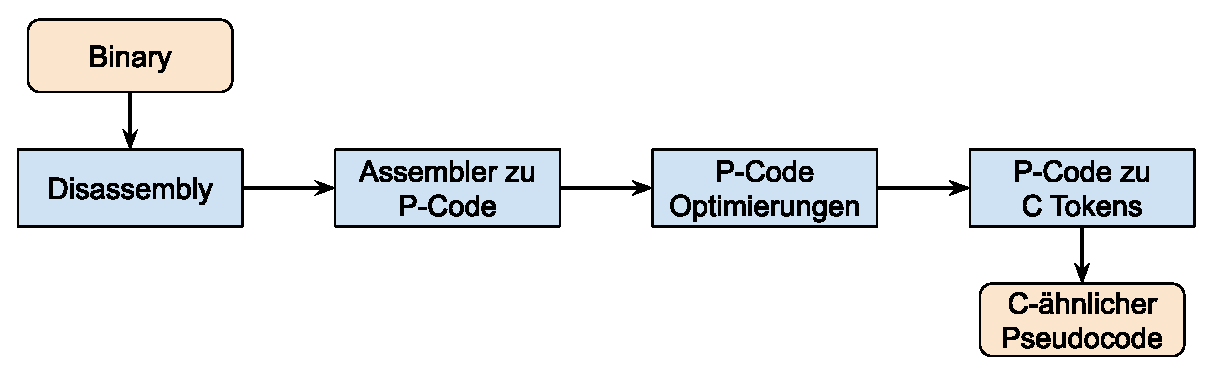
\includegraphics[width=.45\textwidth]{img/DecompilerFunktionsweise.eps}
	\caption{Ghidra Decompiler Funktionsweise Phasen}
	\label{fig:groups}
\end{figure}

\subsection{Disassembly}

In der ersten Phase wird der ausführbare Maschinencode im Binary identifiziert. Eine Herausforderung dabei ist, dass Compiler Daten zusammen mit ausführbarem Maschinencode in derselben ELF Section speichern können. Dies kann zum Beispiel bei Jump Tables der Fall sein \cite{2}. Solche Daten werden auch als Inline Data bezeichnet \cite{2}. Deshalb kann nicht davon ausgegangen werden, dass direkt nach einer Instruktion eine neue Instruktion folgt.

Aufgrund von möglichem Inline Data verwendet Ghidra verschiedene Recursive Descent Algorithmen, um ausführbaren Maschinencode zu identifizieren \cite{3}. Recursive Descent Algorithmen starten an einer gegebenen Maschinencode-Adresse und folgen dann rekursiv dem Control-Flow des Programms \cite{3}. Mit anderen Worten versucht Recursive Descent von einem Einstiegspunkt aus allen möglichen Codepfaden zu folgen um so ausführbaren Maschinencode zu finden. Ghidra verwendet unter anderem den Einstiegspunkt des Programms, die 'main' Funktion, und Cross References um Maschinencode-Adressen für Einstiegspunkte zu finden \cite{3}. Cross References, oder kurz Xrefs, sind Instruktionen und Daten, die über Speicheradressen auf andere Instruktionen oder Daten verweisen \cite{6}.

Während dem Recursive Descent wird Maschinencode zur Assemblersprache disassembled/übersetzt. Ghidra verwendet dafür SLEIGH \cite{7}. SLEIGH ist eine Sprache, welche unter anderem die Instruktionen, Register, und Features eines Prozessors spezifiziert \cite{7}. Jeder von Ghidra unterstützte Prozessor ist durch SLEIGH spezifiziert. 

Bei Recursive Descent Algorithmen kann es vorkommen, dass nicht der komplette ausführbare Maschinencode gefunden wird. Außerdem können Daten fehlerhaft als 'ausführbarer Maschinencode' identifiziert werden. Der Grund dafür sind Unconditional Branching Instruktionen. Zu dieser Art von Instruktionen gehört zum Beispiel 'jmp RAX'. Für diese Instruktionen kann Ghidra durch statische Analyse nicht immer alle möglichen Ziele des Sprungs ermitteln. Um mehr ausführbaren Maschinencode zu finden, verwendet Ghidra weitere Algorithmen und Heuristiken. Zum Beispiel versucht Ghidra mit Hilfe von Heuristiken typische Funktionsprolog und -epilog zu erkennen, um den Anfang von Funktionen zu identifizieren \cite{3}. Die dadurch gefundenen Funktionsanfänge werden als Einstiegspunkte für weiteres Recursive Descent verwendet \cite{3}.

\subsection{Assembler zu P-Code Übersetzung}

Im nächsten Schritt übersetzt Ghidra Assembler Instruktionen zu P-Code \cite{4}. P-Code ist eine Register Transfer Language (RTL) \cite{4}. RTL kann als architekturneutrale Assemblersprache gesehen werden. 

Ghidra übersetzt jeweils eine Assembler Instruktion in eine oder mehrere P-Code Operationen \cite{4}. Diese Übersetzung ist ebenfalls durch die SLEIGH Sprache spezifiziert \cite{7}. P-Code Operationen sind ähnlich wie Assembler Instruktionen. Zum Beispiel gibt es die P-Code Operationen 'INT\_ADD', 'LOAD', und 'BRANCH' \cite{4}.

P-Code Operationen nehmen eine oder mehrere Varnodes als Eingabe und geben optional eine Varnode aus \cite{4}. Eine Varnode ist eine Verallgemeinerung eines Registers oder eines Speicherbereichs \cite{4}. Maschinencode Instruktionen arbeiten mit Registern und Speicher wie dem Stack und Heap. Im Gegensatz dazu arbeiten P-Code Operationen mit Varnodes. Varnodes können somit als architekturneutrale virtuelle Register bzw. Speicher gesehen werden. P-Code Operationen haben keine Nebeneffekte wie zum Beispiel das Setzen von Status Flags.

Um die Zeit zum Starten von Ghidra gering zu halten, werden nicht alle Assembler Instruktionen sofort beim Start von Ghidra zu P-Code und danach zu C übersetzt. Stattdessen arbeitet der Ghidra Decompiler Just-In-Time. Basierend auf der Auswahl des Benutzers wird eine Funktion dekompiliert. Die erste Instruktion der ausgewählten Funktion wird als Einstiegspunkt betrachtet \cite{10}. Vom Einstiegspunkt aus sucht Ghidra nach allen möglichen Pfaden \cite{10}. Die Instruktionen auf diesen Pfaden werden zu P-Code übersetzt \cite{10}.

Das Verwenden von P-Code anstelle von Maschinencode hat mehrere Vorteile für Ghidra's Decompiler. Zum einen müssen die nachfolgenden Analysealgorithmen und Heuristiken nur für eine Sprache entwickelt werden. Ghidra unterstützt verschiedene Prozessoren und verschiedenen Befehlssatzarchitekturen wie x86-64, ARM, und AVR \cite{5}. Ohne diesen Übersetzungszwischenschritt müssten die Analysealgorithmen und Heuristiken an jeden Prozessor und jede Befehlssatzarchitekturen angepasst werden. Durch P-Code muss stattdessen für jeden Prozessor und jede Befehlssatzarchitekturen, welche von Ghidra unterstützt werden soll, eine Übersetzung von allen möglichen Maschinencode Instruktionen zu P-Code implementiert werden. Zum anderen wurde P-Code entworfen, um die Konstruktion von Datenflussgraphen zu erleichtern \cite{4}. Diese Datenflussgraphen werden in den folgenden Analysen benötigt \cite{4}.

\subsection{P-Code Optimierung}

In der dritten Phase wird der P-Code analysiert und nach Lesbarkeit optimiert und transformiert. Diese Phase besteht aus 17 Schritten. Die Schritte 4 bis 9 werden mehrmals wiederholt.

Der P-Code wird optimiert, damit der resultierende Code für den Reverse Engineer einfacher zu verstehen ist \cite{12}. Zum Beispiel werden nicht relevante Details aus dem Code entfernt \cite{12} und Higher-Level Kontrollflussstrukturen wie If-Else Blöcke und Schleifen werden anstelle von 'goto' Anweisungen verwendet \cite{8}. Der optimierte P-Code lässt sich auch besser in C Tokens umwandeln.

% TODO: img here

\begin{description}
\item [1 - Basic Blocks und Control Flow Graph (CFG):] Aus den P-Code Operationen werden Basic Blocks generiert \cite{8}. Diese Basic Blocks werden verwendet, um einen Control Flow Graphen zu erstellen \cite{8} \cite{9}.
\item [2 - Analyse von Funktionsaufrufen:] Ghidra's Decompiler überprüft, ob bereits Informationen für aufgerufene Funktionen vorhanden sind \cite{8}. Zu diesen Informationen gehören zum Beispiel die Anzahl und Datentypen der Funktionsparameter und der Datentyp des Rückgabewerts. Diese Informationen können zum Beispiel von einem Benutzer spezifiziert worden sein. Es gibt auch Datenbanken mit Informationen über Funktionen von bekannten Bibliotheken wie der C Standard Library und OpenSSL \cite{20}. Die Informationen aus diesen Datenbanken können bei Ghidra mit einem Klick importiert werden \cite{20}. Das ist allerdings nur nützlich, wenn das Programm mit diesen Bibliotheken statisch gelinkt ist.
\item [3 - Hinzufügen von P-Code:] Bis jetzt steht dem Decompiler nur der P-Code ab einem bestimmten Einstiegspunkt aus zur Verfügung. Dieser Einstiegspunkt ist die vom Benutzer ausgewählte Funktion. Wenn möglich wird in diesem Schritt neuer P-Code hinzugefügt, damit dem Decompiler in der folgenden Analyse neue relevante Informationen zur Verfügung stehen. Zum Beispiel prüft der Decompiler, ob die Funktion Werte aus dem Speicher liest und ob Ghidra diese Werte bekannt sind \cite{8}. Ist das der Fall, dann werden 'COPY' P-Code Operationen hinzugefügt.
\item [4 - SSA Form:] Der bisherige P-Code wird in Static Single Assignment (SSA) Form gebracht. Für die SSA Form darf jede Varnode nur genau einmal zugewiesen werden \cite{9}. Anstatt den Wert einer Varnode zu überschreiben, wird bei der SSA Form stattdessen eine neue Version dieser Varnode erstellt \cite{12}. P-Code in SSA Form vereinfacht die nachfolgende Datenflussanalyse, weil Varnodes nicht wiederverwendet werden \cite{12}.
\item [5 - Dead Code Elimination:] Dabei wird nicht relevanter P-Code entfernt. Zum Beispiel setzen viele Maschinencode Instruktionen als Nebeneffekt Status Flags, welche für die korrekte Funktion des Programms nicht relevant sind \cite{8}. Außerdem werden unerreichbare P-Code Basic Blocks und Verzweigungsanweisungen, bei denen alle Verzweigungen gleich sind oder die Kondition konstant ist, entfernt \cite{11}.
\item [6 - Typ-Inferenz und -Propagation:] Ghidra's Decompiler verwendet einen Typ-Inferenz Algorithmus, der jede Varnode mit dem Typ versieht, den er für richtig hält \cite{11} \cite{8}. Für jede Varnode sucht der Algorithmus nach P-Code Operationen, an denen diese Varnode als Operand oder als Ausgabe beteiligt ist \cite{11}. Danach wird überprüft, welchen Datentyp die P-Code Operation als Operand bzw. als Ausgabe erwartet \cite{11}. Zum Beispiel erwartet die P-Code Operation 'FLOAT\_ADD' eine Fließkommazahl als Operand. Die Ausgabe ist ebenfalls eine Fließkommazahl. Varnodes, welche bei 'FLOAT\_ADD' als Operand oder Ausgabe beteiligt sind, werden daher vom Typ-Inferenz Algorithmus als Fließkommazahl vermerkt \cite{8}. % TODO: maybe unknown types and user can specify type
Danach werden diese Typen unter anderem über die P-Code Operationen 'COPY', 'LOAD', und 'STORE' weiter propagiert \cite{11}.
\item [7 - P-Code Umschreiben:] In diesem Schritt wird der P-Code in Abstract Syntax Tree (AST) Form verwendet \cite{8}. Der Ghidra Decompiler definiert Regeln, wie ein Teil eines AST umgeschrieben werden kann \cite{8}. Das Ziel dieser Transformationen ist die Vereinfachung des P-Codes \cite{8}. Diese Transformationen sind nicht dazu gedacht, den P-Code zu optimieren. Vielmehr sollen die Transformationen einem Reverse Engineer helfen den P-Code und den daraus resultierenden C Code besser zu verstehen \cite{8}. Aus diesem Grund werden in diesem Schritt auch einige der Compiler-Optimierungen rückgängig gemacht.
\item [8 - Dead Code Elimination durch CFG:] Basierend auf einer Analyze des CFG wird der P-Code von unter anderem nicht erreichbarem Code, leeren Basic Blocks, und nicht verwendeten Branches entfernt \cite{8}.
\item[9 - Wiederherstellen der Kontrollflussstruktur:] In diesem Schritt wird die Kontrollflussstruktur der Funktion aufgebaut. Diese Kontrollflussstruktur ist eine Hierarchie \cite{8}. Die Hierarchie besteht aus Higher-Level Kontrollflussstruktur-Objekten wie If-Else Blöcken, Schleifen, und Switch Anweisungen \cite{8}. Der Ghidra Decompiler kann typische Muster für diese Kontrollflussstruktur-Objekte erkennen.
\end{description}

\noindent
Die Schritte 4 bis inklusive Schritt 9 werden mehrmals wiederholt. Nach jeder Iteration wird der Lower-Level P-Code mehr und mehr zu einer Higher-Level Version des ursprünglichen P-Codes. Die Higher-Level Version kann einfacher in C Tokens übersetzt werden.

\begin{description}
\item [10 - Finale P-Code Transformation:] Dieser Schritt ist ähnlich wie Schritt 7 'P-Code Umschreiben'. Schritt 7 verwendet teilweise Regeln, welche für die finale Ausgabe nicht ideal sind \cite{8}. Stattdessen werden jetzt nur Regeln angewandt, welche die Lesbarkeit der finalen Ausgabe verbessern \cite{8}.
\item [11 - Zusammenführen von Varnodes (Teil 1):] In diesem Schritt wird die Anzahl der verwendeten Varnodes verringert. Wenn möglich, werden dabei mehrere Varnodes zu einer Varnode zusammengeführt \cite{8}. Der daraus resultierende P-Code ist ab sofort auch nicht mehr in SSA Form \cite{8}. Zum Beispiel werden Varnodes durch COPY P-Code Operationen ersetzt \cite{8}. Dabei muss der Decompiler sicherstellen, dass Daten in Varnodes nur überschrieben werden dürfen, wenn diese Daten nicht mehr verwendet werden.
\item [12 - Ausdrücke bestimmen:] Im Vergleich zur Assembler Sprache kann eine Higher-Level Sprache wie C komplexe Ausdrücke haben \cite{12}, wie zum Beispiel 'a = b + 2 * c'. In diesem Schritt werden die finalen Ausdrücke festgelegt \cite{8}.
\item [13 - Zusammenführen von Varnodes (Teil 2):] Weitere Varnodes werden zusammengeführt, weil trotz Teil 1 noch zu viele Varnodes existieren \cite{9}. Im Vergleich zu Schritt 11 ist dieses Zusammenführen mehr spekulativ \cite{8}. Die aus diesem Schritt resultierenden Varnodes werden später im C Code zu Variablen und Funktionsparametern.
\item [14 - Type Casts:] In Schritt 6 hat der Typ-Inferenz Algorithmus jede Varnode mit einem Typ versehen. Nun werden dem Code Type Casts hinzugefügt, damit die finale Ausgabe syntaktisch gültig ist \cite{8}.
\item [15 - Funktionsprototyp:] Der Funktionsprototyp für die vom Benutzer ausgewählte Funktion wird festgelegt \cite{8}. Ein Funktionsprototyp besteht unter anderem aus der Anzahl der Funktionsparametern, den Datentypen der Funktionsparametern, und dem Datentyp des Rückgabewerts \cite{10}. Dafür muss der Decompiler bestimmen, welche Register und/oder Stackbereiche verwendet werden, um Funktionsparameter zu übergeben und den Rückgabewert zurückzugeben. Die Typen für alle Register und relevanten Stackbereiche wurden schon in Schritt 6 durch den Typ-Inferenz Algorithmus bestimmt und sind in den Varnodes gespeichert.
Die Calling Convention gibt an, welche Register und/oder Stackbereiche für die Funktionsparameter und den Rückgabewert in Frage kommen \cite{10}. Ghidra's Decompiler analysiert außerdem, welche der in Frage kommenden Varnodes gelesen werden bevor sie beschrieben werden. Diese werden als Funktionsparameter angesehen. 
\item [16 - Namen für Variablen setzen:] Dabei richten sich die Namen der Variablen nach der Verwendung jeder Variable \cite{8}.
\item [17 - Finale CFG Änderungen:] Abschließend kann die Reihenfolge von Komponenten wie zum Beispiel der Switch Cases geändert werden \cite{8}.
\end{description}
% https://github.com/NationalSecurityAgency/ghidra/blob/da94eb86bd2b89c8b0ab9bd89e9f0dc5a3157055/Ghidra/Features/Decompiler/src/decompile/cpp/docmain.hh

%[W]transforms it until it is structured in a form that can be translated more directly to C tokens.

%- One of the most important aspects of the  decompilation process is the reconstruction of meaningful expressions from these individual instructions.
%- control-flow, data-flow, and prototype information, plus class instances to help with constructing SSA form, structure control-flow, recover jump-tables, recover parameters, and merge Varnodes.

% [D] https://github.com/NationalSecurityAgency/ghidra/blob/4e16b3aa3a649b87a54a6e43a5c01360fd255a83/Ghidra/Features/Decompiler/src/decompile/cpp/coreaction.hh 

% https://www.foo.be/cours/dess-20122013/b/Eldad_Eilam-Reversing__Secrets_of_Reverse_Engineering-Wiley(2005).pdf
% book talks about Primitive Data Types, Complex Data Types

\subsection{P-Code zu C Tokens}

Aus dem optimierten P-Code und den zusätzlichen Informationen über den Funktionsprototyp, dem CFG, den Higher-Level Kontrollflussstruktur-Objekten, und den festgelegten Ausdrücken werden die finalen C Tokens generiert \cite{8}. Beispiele für C Tokens werden in Figure \ref{fig:ctokens} gezeigt.

\begin{figure}[!h]
	\centering
	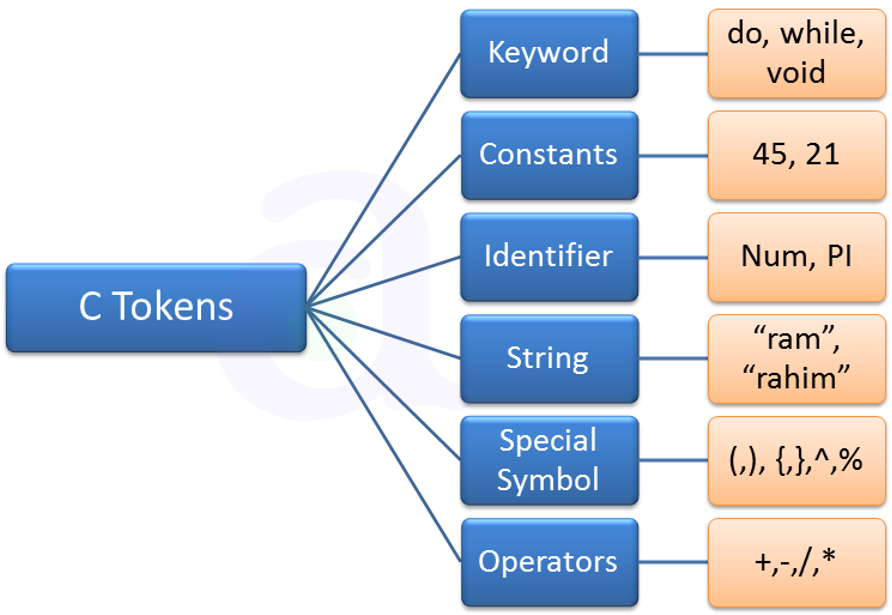
\includegraphics[width=.45\textwidth]{img/ctokens.png}
	\caption{C Tokens Kategorien und Beispiele}
	\label{fig:ctokens}
\end{figure}


%[W] % http://chasekanipe.com/writeups/ghidra.pdf
%> tends to fail (at least in 2019) at obfuscationand fails at type identification where there is heavy compiler optimization. but i guess all decompilers have issues with that.

% !! https://github.com/NationalSecurityAgency/ghidra/blob/master/Ghidra/Features/Decompiler/src/decompile/cpp/docmain.hh

%\section{Arbeiten mit dem Ghidra Decompiler}

%TODO: 1 para

% subsection info an benutzer, e.g. confidence indicatior thing
% wann decompiler allgemein nicht so gut. dann vllt auf andere RE dinge konzentrieren oder mit einplanen dass source verstehen länger dauert
% difference decompileroutput vs 'normal' c code?



\section{Typische Probleme bei der Dekompilation}

Bei der Kompilierung gehen Informationen verloren \cite{12}. Zu diesen verlorenen Informationen gehören unter anderem Variablennamen, Variablentypen, Kommentare, und die Deklarationen von Datenstrukturen \cite{12}. Es gibt keinen klar definierten Prozess, um die verlorenen Informationen mit 100\%iger Sicherheit wiederherzustellen. Das macht Dekompilation nicht unmöglich, aber der Decompiler muss an mehreren Phasen und Schritten im Übersetzungsprozess von Maschinencode zu C Heuristiken einsetzten. Mit anderen Worten muss Ghidra Annahmen treffen. Diese Annahmen können falsch sein. Deshalb kann die Ausgabe des Decompilers falsch sein. Manche Informationen können auch nicht wiederhergestellt werden. Dadurch wird es für den Reverse Engineer schwieriger, den resultierenden C-Code zu verstehen.

Aus diesen Gründen kann der Benutzer die Dekompilation verbessern, indem der Benutzer Ghidra mehr Informationen zur Verfügung stellt. Ghidra weist den Benutzer auf nicht wiederhergestellte Informationen, Fehler, und auf mögliche Fehler hin. Dazu gehört zum Beispiel, wenn Maschinencode nicht disassembled werden konnte oder wenn der Typ einer Variablen oder eines Funktionsparameters nicht wiederhergestellt werden konnte. Diese Hinweise werden in dieser Sektion vorgestellt.

Der Ghidra Decompiler ist interaktiv. Benutzer können sogenannte Program Annotations (dt. Programm Anmerkungen) hinzufügen, ändern, und löschen \cite{1}. Dabei wird die Ausgabe des Ghidra Decompilers dynamisch aktualisiert. Diese Annotations werden ebenfalls in dieser Sektion vorgestellt. % annotations als 2nd part? oder neue subsection?

\subsection{Instruktionen als Daten identifiziert}

Ghidra's Decompiler verwendet für das Disassembly verschiedene Recursive Descent Algorithmen und Heuristiken. Trotzdem können ausführbarere Maschinencodeinstruktionen fälschlicherweise als Daten identifiziert werden. Aus diesem Grund können Benutzer von Ghidra diese Speicherbereiche manuell als 'ausführbarer Maschinencode' markieren. Dadurch können diese Speicherbereiche ebenfalls dekompiliert werden. 

\subsection{Disassembly schlägt fehl}

Wenn der Decompiler Speicherbereiche von Maschinencode zu Assembler Instruktionen übersetzen soll, dann kann dies fehlschlagen. Ghidra's Decompiler gibt in diesem Fall einen 'Bad Instruction' Error aus.

Das Fehlschlagen kann verschiedene Gründe haben. Ein Grund kann sein, dass ein Speicherbereich verschlüsselt oder komprimiert ist und nur zur Laufzeit entschlüsselt oder dekomprimiert wird. Ghidra's Entropie Indikator kann einen Hinweis darauf geben, welche Speicherbereiche verschlüsselt oder komprimiert sind \cite{14}. In diesem Fall könnte man den Code in einer sicheren Umgebung ausführen und den Inhalt des Prozess RAMs speichern und mit Ghidra analysieren. In Figure \ref{fig:entropy} befindet sich der Entropie Indikator auf der rechten Seite. Je nach der Entropie zeigt der Indikator für einen Speicherbereich schwarz (wenig Entropie), gelb, oder rot (hohe Entropie) an.

\begin{figure}[!h]
	\centering
	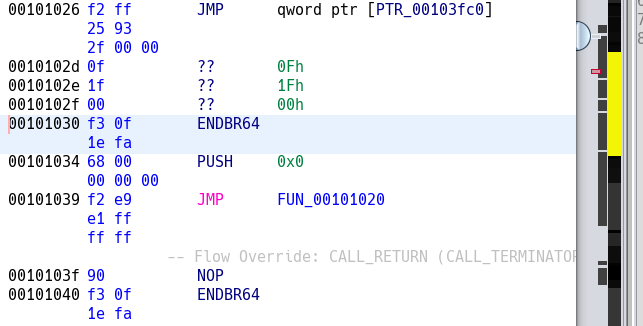
\includegraphics[width=.45\textwidth]{img/entropy.png}
	\caption{Ghidra Entropie Indikator}
	\label{fig:entropy}
\end{figure}

% vielleicht irgendwo entropy; https://dannyquist.github.io/gootkit-reversing-ghidra/
%	> entropy indikator für welche teile der executable encrypted oder compressed sind. die kann der ghidra decompiler nicht dekompilieren. MC muss entschlüsselt sein bevor der CPU ihn ausführen kann. also kann man evtl. exe ausführen und während ausführung process dump machen;

\subsection{Funktion wird nicht erkannt}

Benutzer können eine Instruktion auswählen. Der Decompiler dekompiliert daraufhin die Funktion, zu der die ausgewählte Anweisung gehört \cite{13}. Allerdings kann der Decompiler die Grenzen dieser Funktion nicht immer erkennen \cite{1}. Mit anderen Worten: Die erste und letzte Instruktion dieser Funktion zu bestimmen ist nicht immer möglich.

Ghidra liefert in diesem Fall trotzdem eine Ausgabe \cite{1}. Die erste Instruktion wird ausgewählt, indem der Kontrollfluss von der ausgewählten Instruktion aus zurückverfolgt wird, bis ein Basic Block gefunden wird, dessen eingehende Kanten nur 'CALL' Instruktionen sind \cite{13}. Um die letzte Instruktion auszuwählen, wird dem Kontrollfluss gefolgt bis eine Instruktion mit Terminator Semantik, wie zum Beispiel 'RETURN', gefunden wird \cite{13}. Um den Benutzer anzuzeigen, dass die Grenzen der Funktion nicht ermittelt werden konnten, wird der Hintergrund des Decompiler Ausgabefensters grau und der Funktionsname erhält das Präfix 'UndefinedFunction\_' \cite{13}. Benutzer von Ghidra können die Grenzen der zu dekompilierenden Funktion auch selbst festlegen \cite{1}.


\subsection{Funktion ohne Return}

Manche Funktionen sind non-returning. Das bedeutet, dass nach dem Aufruf einer non-returning Funktion der Rest der Aufruferfunktion nicht mehr ausgeführt wird. Non-returning Funktionen sind zum Beispiel Funktionen, die das Programm beenden, wie 'exit()', und Funktionen mit einer Endlosschleife.

Ein Compiler kann non-returning Funktion erkennen und als Optimierung den Rest der Aufruferfunktion entfernen. Dabei wird auch die Instruktion mit Terminator Semantik, wie zum Beispiel 'RETURN', in der Aufruferfunktion entfernt.

Wenn Ghidra nicht weiß, dass eine Funktion non-returning ist, dann versucht der Ghidra Decompiler den Maschinencode nach der 'CALL' Instruktion zu dekompilieren \cite{15}. Dieser Maschinencode ist nicht Teil der Funktion und kann Daten enthalten, wodurch die Dekompilierung fehlschlägt oder Daten fälschlicherweise als Instruktionen interpretiert werden.

Ghidra's Decompiler versucht non-returning Funktion zu erkennen \cite{15}. Zum einen hat Ghidra eine Liste von Funktionsnamen, welche üblicherweise non-returning Funktionen sind \cite{15}. Zu diesen Funktionsnamen gehören 'exit' und 'abort'. Zum anderen werden verschiedene Heuristiken verwendet, die nach Indikatoren suchen, dass eine Funktion non-returning ist \cite{15}. Ein Indikator ist zum Beispiel, dass nach einer CALL Instruktion der Funktionsepilog einer anderen Funktion ist.

Benutzer können einen 'Function Non-return Threshold' angeben. Wenn die Anzahl der Indikatoren für eine Funktion höher als der Threshold ist, dann wird die Funktion als non-returning klassifiziert \cite{21}.

Trotzdem kann eine Funktion falsch klassifiziert werden \cite{15}. Aus diesem Grund können Benutzer eine Funktion auch manuell als 'No Return' markieren. Das wird in Figure \ref{fig:noreturn} gezeigt. Wenn eine Funktion fälschlicherweise als non-returning klassifiziert worden ist, z.B. wenn ein zu niedriger Threshhold gewählt worden ist, dann können Benutzer die 'No Return' Markierung entfernen. Wenn eine Funktion nicht in allen Fällen non-returning ist, dann können Benutzer einzelne 'CALL' Instruktionen durch sogenannte Flow Overrides als 'CALL\_RETURN' kennzeichnen \cite{1}. Ein Beispiel dazu ist in Figure \ref{fig:callreturn} zu sehen. Der Ghidra Decompiler berücksichtigt alle 'No Return' Markierungen und Flow Overrides.

\begin{figure}[!h]
	\centering
	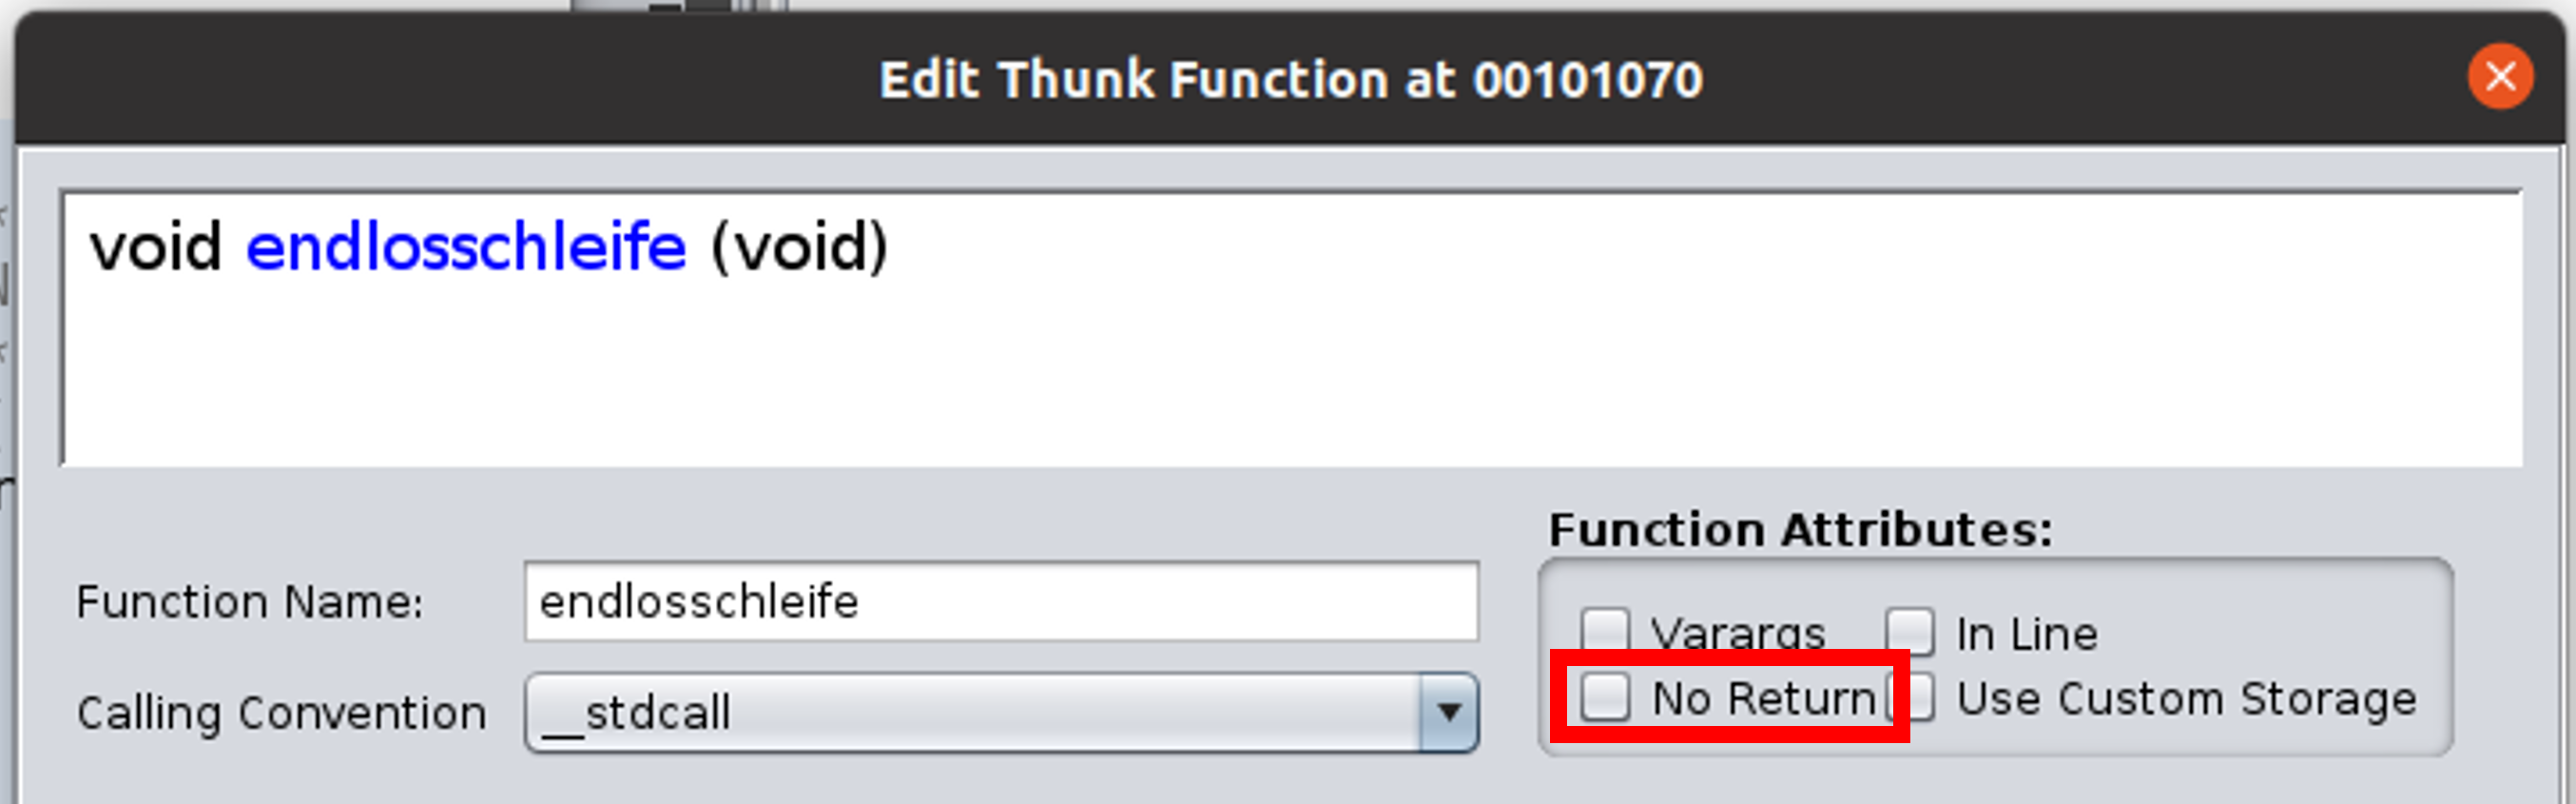
\includegraphics[width=.45\textwidth]{img/noreturnmarkierung.png}
	\caption{No Return Funktion Markierung}
	\label{fig:noreturn}
\end{figure}

\begin{figure}[!h]
	\centering
	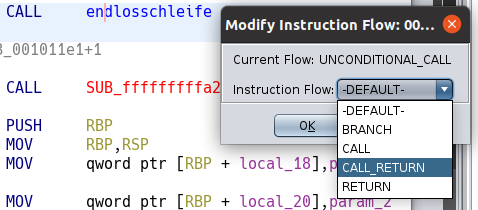
\includegraphics[width=.45\textwidth]{img/callreturn.PNG}
	\caption{Flow Overrides}
	\label{fig:callreturn}
\end{figure}

\subsection{Datentyp}

Der Typ-Inferenz Algorithmus kann nicht in allen Fällen die Datentypen aller Variablen, Funktionsparametern, und der Rückgabewerte bestimmen. Wenn ein Datentyp nicht bestimmt werden kann, dann wird der Datentyp in der Decompilerausgabe als 'undefined' angegeben \cite{1}. Benutzer können die Datentypen spezifizieren und Datentypen ändern \cite{1}. 

Der Typ-Inferenz Algorithmus hat oft Probleme, bei nicht primitiven Datentypen den korrekten Datentyp wiederherzustellen. Zu den nicht primitiven Datentypen gehören unter anderem Structs, Enums, und Klassen. Zum Beispiel werden Structs oft als Array klassifiziert. Die Ausgabe des Decompilers ist dann nicht falsch. Allerdings ist die Ausgabe dann oft nicht gut lesbar. Ein Benutzer kann deshalb auch benutzerdefinierte Datentypen wie Structs, Enums, und Klassen definieren und als Typen verwenden \cite{15}.

% 'undefinedX'

\subsection{Funktionsprototyp}

Der Decompiler kann auch Fehler bei der Anzahl der Funktionsparameter machen. Zusätzlich zu den Typen der Funktionsparameter und des Rückgabewerts können Benutzer ebenfalls die Anzahl der Funktionsparameter ändern \cite{1}. % tatsächlich 1 arg aber 2 angegeben

\subsection{Anti-Decompile Technik}

Die zu dekompilierende Funktion kann Techniken verwenden, welche das Dekompilieren erschweren oder verhindern sollen. Zum Beispiel kann der Code eine bedingte Verzweigungsanweisung haben, dessen Bedingung immer Wahr ist \cite{15}. Es kann aber schwierig sein, das statisch herauszufinden \cite{15}. Das bedeutet, dass der Falsch-Pfad durch Dead Code Elimination nicht entfernt wird und ebenfalls dekompiliert wird. Der Falsch-Pfad kann dann Instruktionen enthalten, die den Decompiler absichtlich zu Fehlern führen soll \cite{15}. Zum Beispiel könnte man dort eine 'JUMP' Instruktion einbauen, die zu einer Adresse springt, an der sich Daten befinden. Für solche Fälle können Benutzer das sogenannte Patch Instruction einsetzen \cite{15}, um zum Beispiel eine bedingte Verzweigungsanweisung durch eine 'JUMP' Instruktion zum Wahr-Pfad zu ersetzen. 

Allerdings kann es auch für Benutzer schwierig sein, toten Code zu erkennen. Dafür könnte man den Code in einer sicheren Umgebung ausführen und analysieren, welche Basic Blocks ausgeführt werden.

\subsection{Data Mutability}

Data Mutability beschreibt, wie sich Daten in einem Speicherbereich während der Ausführung verändern können \cite{1}. Ein Speicherbereich ist eine einzelne Variable oder ein größerer Speicherblock \cite{1}.

In Ghidra werden die Daten in einem Speicherbereich entweder als 'Normal', 'Constant', oder als 'Volatile' klassifiziert \cite{1}. 'Normal' bedeutet, dass sich die Daten ändern können \cite{1}. Das passiert in diesem Fall allerdings nur, wenn eine Instruktion explizit die Daten überschreibt \cite{1}. 'Constant' Daten ändern sich nicht \cite{1}. Als 'Volatile' klassifizierte Daten können sich ändern, auch wenn keine Instruktion die Daten explizit überschreibt \cite{1}. Das ist zum Beispiel bei Shared Memory oder bei Memory Mapped I/O der Fall.

Wenn der Ghidra Decompiler mit Daten arbeitet, die nicht als 'Volatile' klassifiziert sind, kann er bestimmte Vereinfachungen nicht einsetzen \cite{15}. Benutzer können die Mutability von Speicherbereichen ändern \cite{1}.

\subsection{Probleme im Code}

Ghidra's Decompiler kann Variablen mit dem Präfix 'in\_' und 'unaff\_' versehen \cite{15}. In diesem Fall denkt der Decompiler, dass die Variable einen nicht initialisierten Wert enthält, der verwendet wird \cite{15}. Mit anderen Worten: Die Variable wird verwendet, bevor in sie geschrieben wird. 

Das kann ein Fehler im Programm oder ein Fehler des Decompilers sein. Eine mögliche Ursache ist, dass ein Funktionsprototyp falsch ist \cite{15}. Zum Beispiel könnte ein Rückgabewert eine falsche Größe haben \cite{15}.

Die Ausgabe des Decompilers kann P-Code enthalten. In diesem Fall konnte der Decompiler diesen P-Code nicht in C Tokens umwandeln \cite{15}.


\bibliographystyle{plainurl}
\bibliography{\jobname}

\end{document}

%%  LocalWords:  endnotes includegraphics fread ptr nobj noindent
%%  LocalWords:  pdflatex acks